\documentclass[11pt]{report}
\usepackage[utf8]{inputenc}
\usepackage[T1]{fontenc}
\usepackage[unicode=true]{hyperref}
\usepackage{lmodern}
\usepackage[french]{babel}

%%% PAGE DIMENSIONS
\usepackage{geometry}
\geometry{a4paper}
\geometry{top=2.5cm, bottom=2.5cm, left=4.5cm , right=3.5cm}
\usepackage{graphicx}


%%% PACKAGES
\usepackage{booktabs} % for much better looking tables
\usepackage{array} % for better arrays (eg matrices) in maths
\usepackage{paralist} % very flexible & customisable lists (eg. enumerate/itemize, etc.)
\usepackage{verbatim} % adds environment for commenting out blocks of text & for better verbatim
\usepackage{subfig} % make it possible to include more than one captioned figure/table in a single float
\usepackage{amssymb,amsmath}
\usepackage{xcolor}
\usepackage{sistyle}
\usepackage{shorttoc}
\usepackage{titlesec}
\usepackage{titletoc}

\hypersetup{breaklinks=true,
            pdfauthor={Thibault Deutsch (deutsc\_t); Rémy Bernier (bernie\_r); Marc Fresne (fresne\_m); Anthony Belthier (belthi\_a)},
            pdftitle={Rapport de projet},
            colorlinks=true,
            citecolor=blue,
            urlcolor=blue,
            linkcolor=black,
            pdfborder={0 0 0}}

\setlength{\parskip}{6pt plus 2pt minus 1pt}
\setlength{\emergencystretch}{3em}  % prevent overfull lines

\setcounter{secnumdepth}{3}
\setcounter{tocdepth}{4}
\renewcommand{\thechapter}{\Roman{chapter}}
\renewcommand{\thesection}{\arabic{section}.}
\renewcommand{\thesubsection}{\arabic{section}.\arabic{subsection}}
\renewcommand{\thesubsubsection}{\arabic{section}.\arabic{subsection}.\arabic{subsubsection}}

\usepackage{fancyhdr} % This should be set AFTER setting up the page geometry
\pagestyle{fancy}
\fancyhead[L]{Emagine Studio}
\fancyhead[C]{}
\fancyhead[R]{Troma}

\title{Rapport de projet}
\author{Thibault Deutsch (deutsc\_t) \and Rémy Bernier (bernie\_r) \and Marc Fresne (fresne\_m) \and Anthony Belthier (belthi\_a)}
\date{12 juin 2014}

\dottedcontents{chapter}%
  [\dimexpr 10mm]
  {}
  {\dimexpr 10mm}
  {3.2mm}

\dottedcontents{figure}%
  [\dimexpr 15mm]
  {}
  {\dimexpr 15mm}
  {3.2mm}

\begin{document}
\renewcommand{\labelitemi}{$\bullet$}

\begin{titlepage}
\newcommand{\HRule}{\rule{\linewidth}{0.5mm}} % Defines a new command for the horizontal lines, change thickness here

%----------------------------------------------------------------------------------------
%	LOGO SECTION
%----------------------------------------------------------------------------------------
\flushright
\includegraphics[width = 4.5cm]{EPITA.png}\\[0.5cm] % Include a department/university logo - this will require the graphicx package

%----------------------------------------------------------------------------------------
%	HEADING SECTIONS
%----------------------------------------------------------------------------------------
\textsc{\Large Rapport de projet}\\[0.15cm] % Major heading such as course name
\textsc{\large 1\ier{} année du cycle préparatoire}\\[3cm] % Minor heading such as course title

%----------------------------------------------------------------------------------------
%	TITLE SECTION
%----------------------------------------------------------------------------------------
\center
\HRule \\[0.5cm]
{\Huge \bfseries Troma}\\[0.3cm] % Title of your document
\textsc{\Large Jeu vidéo en 3D}\\[0.1cm]
\large Réalisé par le groupe \emph{Emagine Studio}\\[1.5cm]
\large 12 juin 2014\\[0.1cm]
\HRule \\[2cm]

\includegraphics[width = 4cm]{eie.png}\\[1cm]

\Large
\textbf{Thibault Deutsch} (\emph{deutsc\_t}) \\
\textbf{Rémy Bernier} (\emph{bernie\_r}) \\
\textbf{Marc Fresne} (\emph{fresne\_m}) \\
\textbf{Anthony Belthier} (\emph{belthi\_a})\\[2cm]

%----------------------------------------------------------------------------------------
\vfill % Fill the rest of the page with whitespace

\end{titlepage}

\newpage
\pagenumbering{arabic}
\shorttableofcontents{Sommaire}{1}

\chapter*{Introduction}

Ce document est le rapport de la soutenance finale. Il a pour but de présenter une synthèse sur le travail fournit par l'équipe en charge du projet. Cette équipe est formée de quatre étudiants en première année du cycle préparatoire de l'EPITA : Anthony BELTIER (beltie\_a), Rémy BERNIER (bernie\_r), Thibault DEUTSCH (deutsc\_t) et Marc FRESNE (fresne\_m).

Le projet consiste en la réalisation d'un logiciel de notre choix, en C\# ou en CAML. Le développement s'est déroulé sur une période d'environ 6 mois, découpée en 4 étapes : la remise d'un cahier des charges, une soutenance de présentation, une soutenance intermédiaire de démonstration des avancées et une soutenance finale pour présenter le projet achevé. Il a pour but l'apprentissage du développement, du travail de groupe, et de la réponse à une demande précise en un temps donné. L'objectif est d'offrir aux étudiants l'occasion de réaliser un projet dans des conditions similaires à celles qui régissent le monde professionnel.

Nous avons choisi de réaliser un jeu vidéo car c'est un domaine que nous apprécions et que nous pensions que cela faciliterait la réalisation par le côté ludique du projet. Nous avons opté pour l’utilisation du C\# car il s’agit d’un langage particulièrement adapté à ce type de projet. 

\begin{figure}[htbp]
\centering
\includegraphics[width=8cm]{troma.png}
\caption{Logo de notre jeu}
\end{figure}

Nous nous sommes orientés sur un jeu en 3D car cela représentait un véritable défi pour l'ensemble du groupe. Le style de jeu retenu est un jeu de tir en vue subjective\footnote{FPS : First Person Shooter} car c'est un type de jeu que nous apprécions mais aussi car la demande dans l'industrie du jeu vidéo ne cesse de croître. La thématique de notre jeu est la seconde Guerre Mondiale par soucis d'originalité, en effet l'offre s'oriente aujourd'hui principalement vers des univers futuristes, mais aussi afin d'être en accord avec le soixante dixième anniversaire du débarquement de Normandie. Notre jeu se découpe principalement en deux parties : un mode d'entrainement en solo et un mode multijoueur.

Une fois le style de notre jeu défini, il nous fallait un nom pour le projet. C'est en réfléchissant longuement sur la seconde Guerre Mondiale que nous avons pensé au mot ``traumatisme''. Ce mot représente l'effet de la guerre sur une génération entière. Cependant ce mot était un peu trop long. Nous avons donc poussé notre réflexion plus loin et sommes tombés sur le mot ``trauma''.

\begin{quote}
``Un trauma est une blessure physique ou psychique infligée à l'organisme, ou la lésion locale qui en résulte. Le traumatisme renvoie quant à lui aux conséquences locales ou générales du trauma.'', \emph{Wikipédia}
\end{quote}

Comme le montre cette définition, les deux mots sont intimement liés. Mais nous sommes allés encore un peu plus loin. Nous avons décidé de surpasser l'orthographe du mot. Ainsi notre jeu s'appelle Troma. Court, évoquant, surprenant ! On ne pouvait pas trouver mieux. A partir de là, le projet pouvait commencer. 

La répartition des tâches est présentée dans le tableau en figure~\ref{tab}.

\colorlet{darkgreen}{green!60!black}

\begin{figure}[htbp]
\centering
\begin{tabular}{ | c || c | c | c | c | }
\hline Tâches & Thibault & Rémy & Marc & Anthony \\
\hline Modélisation & & & \textcolor{darkgreen}{X} & \\
\hline Moteur graphique & \textcolor{darkgreen}{X} & & \textcolor{darkgreen}{X} & \\
\hline Moteur physique & & \textcolor{darkgreen}{X} & & \textcolor{darkgreen}{X} \\
\hline Menu & & \textcolor{darkgreen}{X} & & \textcolor{darkgreen}{X} \\
\hline Réseau & \textcolor{darkgreen}{X} & & \textcolor{darkgreen}{X} & \textcolor{darkgreen}{X} \\
\hline Gameplay & \textcolor{darkgreen}{X} & \textcolor{darkgreen}{X} & & \\
\hline Audio & & \textcolor{darkgreen}{X} & & \textcolor{darkgreen}{X} \\
\hline Site web & \textcolor{darkgreen}{X} & \textcolor{darkgreen}{X} & & \\
\hline
\end{tabular}
\caption{Répartition des tâches sur l'ensemble de la durée du projet}
\label{tab}
\end{figure}

Vous trouverez dans la suite de ce rapport une présentation détaillée sur les différentes dimensions du développement ainsi qu'une synthèse personnelle de cette expérience.

\chapter{Modélisation}

Un jeu en 3D tel qu'un FPS se base sur un univers complet plus ou moins réaliste. Afin d'offrir un tel univers il est important de poser des bases indispensables à la conception et à la création de celui-ci. Dans un premier temps il faut choisir l’environnement ainsi que le contexte dans lequel se déroulera le jeu.

Nous avons choisi un thème historique : la seconde Guerre Mondiale. Cela implique donc de respecter un minimum le contexte ainsi que les décors pour rendre le jeu crédible et agréable à jouer. Par ailleurs notre jeu disposant de deux modes, un solo et un multijoueur, avec des objectifs relativement différents, nous avions un minimum de deux cartes à modéliser.  Toutes les modélisations ont été réalisées à l’aide du logiciel Blender et les textures à l’aide de Gimp.  Ces deux logiciels sont libres et gratuits.

\section{La conception}

La conception est l’étape de création d’une liste des objets à modéliser ainsi que d’élaboration des plans pour les différentes cartes et bâtiments. Comme indiqué dans l’introduction nous avions besoin de deux cartes, l’une destinée au mode solo, l’autre au mode multi-joueurs. La première sera évidemment plus petite que la deuxième mais aussi différente d’un point de vue décors.

La carte solo prend place aux Etats-Unis dans un milieu rural.

La carte multijoueur prend place en Europe dans un milieu urbain. Elle est inspirée d’une partie de Cracovie, Pologne. Cependant pour des raisons de jouabilité nous avons modifié quelque peu sa structure.

\section{Les techniques de modélisation}

Une fois la conception terminée, la modélisation peut commencer. Afin de ne pas trop alourdir le jeu et ainsi conserver de bonne performance, chaque objet doit être simplifié au maximum. En effet les objets sont formés à partir de sommets\footnote{Vertices}, plus leur nombre est grand plus le fichier est gros et plus les procédures de traitement de ce fichier sont longues.

\subsection{Les bâtiments}

Pour ce faire, chaque bâtiment a été réduit en deux parallélépipèdes, un carré ou rectangle pour les murs, et un trapézoïdal pour le toit. Ensuite il a suffi de modéliser différents modèles de porte ou de fenêtre et de les associer à ces bâtiments.

\begin{figure}[htbp]
\centering
\includegraphics[width=8cm]{batiment.png}
\caption{Modélisation d'un bâtiment}
\end{figure}

Par ailleurs il est important que le maillage\footnote{Mesh} soit découpé en plusieurs objets si la partie au sol n'est pas strictement rectangulaire. En effet cela facilite énormément la gestion des collisions. Des explications plus détaillées seront fournies à la section correspondante.

\subsection{Le personnage et les armes}

Pour des modèles aussi complexes il est encore plus important de maintenir le nombre de sommets aussi bas que possible. Une technique de modélisation pour y arriver est d’utiliser des formes rectangulaire afin d’obtenir une silhouette grossière de l’objet considéré puis d’utiliser des ``modifiers'' pour déformer le maillage et le rapprocher de la forme souhaitée. La réalisation de la silhouette est possible sans être un as du dessin en s’appuyant sur une image qu’il est possible d’avoir en arrière-plan. Cette technique s’appelle ``blueprint'' (en référence au plan de couleur bleu).

\section{Les textures}

Les textures sont de simples images utilisées pour habiller les modèles. Afin de pouvoir se servir de ces images sur un volume il est nécessaire d’avoir une sorte de patron. Cette étape a pour nom l’UV mapping et se décompose en 3 actes : l’édition des lignes de découpe, le dépliage et enfin la création de la texture en fonction du plan obtenu.

\subsection{Le découpage}

Cette étape n’est pas toujours indispensable, surtout pour des modèles très simples. Cependant elle permet de délimiter avec certitude les différentes surfaces qui apparaitront sur la carte UV. Les lignes de découpe sont appelées ``seems'', pour les créer il faut simplement sélectionner les arêtes concernées. 

\begin{figure}[htbp]
\centering
\includegraphics[width=8cm]{seems.png}
\caption{Capture d'écran de blender montrant les ``seems''}
\end{figure}

\subsection{Le dépliage}

Il s’agit de la mise à plat des surfaces du volume selon des lignes de découpe, créées manuellement ou par l’ordinateur. Cette carte fait correspondre ses coordonnées U et V aux coordonnées dans l’espace X, Y et Z de chaque point. Il existe plusieurs options de dépliage qui ne seront pas abordées dans le rapport. En effet avec un découpage adéquat un dépliage classique offre de bon résultat. 

Une fois celui-ci effectué on obtient le patron du modèle. Il est éditable depuis blender, c’est-à-dire que l’on peut modifier si besoin la position des différentes faces. Cela permet d’ajuster la position des différentes faces selon le résultat souhaité. Par ailleurs il est aussi possible de voir à quel point ont été déformé les faces lors du dépliage. Cette option permet de corriger des déformations trop importantes responsables de décalage ou d’artefact sur le modèle texturé.

\begin{figure}[htbp]
\centering
\includegraphics[width=8cm]{unwrap.png}
\caption{Capture d'écran de blender montrant le dépliage}
\end{figure}

\subsection{Export et édition}

Lorsque la carte parait convenable, il convient de l’exporter pour pouvoir l’utiliser dans un logiciel de retouche d’image. Elle permet de construire une texture qui s’ajustera parfaitement sur le modèle.  Cependant, si la texture s’affiche en respectant le découpage, elle n’est pas toujours du bon côté. Chaque surface est définie par les points qui la constituent mais aussi par un vecteur normal et l’image sera affichée selon le sens de celui-ci. Ainsi il arrive que lors de la création du modèle certains de ces vecteurs soient dirigés dans la mauvaise direction.

Heureusement blender permet d’afficher ces vecteurs et de les inverser facilement. Si tous les vecteurs sont dans le bon sens le modèle est prêt.

\section{Les animations}

Les bâtiments et les divers éléments du décor sont statiques et de ce fait n’ont pas besoin d’être animé. Mais ce n’est pas le cas des armes ou bien des personnages. Pour obtenir les animations, deux techniques sont possibles. Soit réaliser le modèle et programmer manuellement les mouvements des différents meshes depuis Visual Studio.

Soit réaliser les animations depuis blender et les exporter pour les lire ensuite. Par commodité Marc a choisi d’utiliser la seconde méthode. La création d’une animation en utilisant des os\footnote{Bones} s’effectue en trois étapes : le ``rigging'', le ``skinning'', et enfin l’enregistrement de l’animation. Utiliser une armature composée d'os permet d'animer des modèles complexes, par exemple le personnage, en modifiant le maillage en fonction du mouvement.

\subsection{Première étape : le ``rigging''}

Le rigging consiste à créer une armature, un squelette, et à organiser une hiérarchie entre les os.
Il s’agit de disposer les os de façon à être capable d’effectuer les mouvements désirés et d’indiquer la dépendance des os entre eux.

\begin{figure}[htbp]
\centering
\includegraphics[width=11cm]{rigging.png}
\caption{Illustration du ``rigging''}
\end{figure}

Un os peut avoir un parent ou non, et peut lui-même être père ou non. Si l’os est père d’un autre alors le mouvement du père entraine le mouvement du fils.

\subsection{Deuxième étape : le ``skinning''}

Le skinning consiste à affecter à chaque os les points du maillage sur lesquels il aura une influence, c’est la notion de poids d’influence\footnote{Weight}. La valeur de ce poids est comprise entre 0 et 1, 0 étant l’influence nulle et 1 l’influence maximale.

Blender offre plusieurs possibilités sur ce point :

\begin{itemize}
\item Soit affecter automatiquement les points du maillage aux os en  fonction de leur enveloppe, c’est à dire leur rayon d’action.
\item Soit affecter automatiquement les points du maillage aux os en  fonction de leur position par rapport aux os.
\item Soit manuellement. Là encore deux solutions sont possibles :
\begin{itemize}
	\item Sélection de points et affectation a un ``vertex group'', comprendre groupe de point influencé par l’os
	\item Selection par ``Weight Painting'', c’est le même principe sauf qu’au lieu de sélectionner les points du maillage, il suffit de ``peindre'' la surface qui dépendra de l’os.
\end{itemize}
\end{itemize}

\begin{figure}[htbp]
\centering
\includegraphics[scale=0.8]{skinning.png}
\caption{Skinning selection maillage à gauche, Weight Painting à droite}
\end{figure}

Les deux premières méthodes de skinning ne sont à utiliser que pour des modèles très simple. Marc n’a donc pas pu les utiliser.

\noindent\textbf{N.B.} Il est très important que tous les points dépendent d’au moins un os. Une solution pour vérifier que tous les points ont un poids est de parcourir les ``vertex groups'' en mode Weight Painting et de chercher une région restée bleue tout le long du parcours.

\subsection{Troisième étape : la création de l’animation}

Une fois le squelette construit et les dépendances avec le maillage assignées, il faut maintenant définir les mouvements qui composeront l’animation.

Pour modifier le positionnement des os et que cela ait une influence sur le maillage il faut se placer en ``pose mode''.  Blender permet de diviser l’écran en plusieurs zones pour pouvoir travailler sur différents aspects en même temps. Par défaut sous la vue 3D il y a une zone où le mode ``TimeLine'' est activé. Il s’agit d’un axe représentant le temps sur lequel on peut se déplacer, et servant à indiquer les différents paramètres du modèle en fonction du temps.

C’est grâce a cette ``TimeLine'' que l’on réalise une animation. Il suffit de se placer a un instant t et d’enregistrer les informations voulues pour les lier. Ces instants sont appelés KeyFrames. Ainsi pour l’animation de la cible, à l’instant t1 la cible est relevée, à l’instant t2 la cible est baissée.

Grace à Blender ces deux instants suffisent pour que la cible se baisse et passe de la position-rotation de l’instant t1 a celle de l’instant t2 de manière progressive durant le temps qui sépare ces deux instants. En effet celui-ci va calculer les différents paramètres  à appliquer au modèle à chaque instant pour que l’animation soit fluide.

Une fois l’action créée, il n’y a plus qu’à exporter le modèle.

\subsection{Exploitation des animations dans XNA}

Une fois le modèle et l’animation créés et exportés, il va falloir récupérer ces informations pour être capable de lancer l’animation dans XNA. Toutes les informations concernant le modèle sont conservées sous forme de matrice (par exemple la position des points) ou de tableau (par exemple le poids des points, os). 
Par défaut le ModelProcessor d’XNA pour les fichiers .X ne récupère pas d’information concernant les animations. Il a donc fallu utiliser un autre ContentProcessor pour récupérer les informations de skinning, les  KeyFrames ainsi que la relation entre les os.

Pour ce faire nous avons récupéré l'exemple nommé ``Skinned Model'' mis à disposition par Microsoft\footnote{\url{http://xbox.create.msdn.com/en-US/education/catalog/sample/skinned_model}}.

Une fois l’extension du Model Processor intégrée à notre code, nous étions en mesure de lancer des animations et de les afficher. Cependant nous nous heurtons à quelques problèmes lié à la gestion du temps des animations.

\section{Les finitions}

Une fois les modèles et leur texture créés on dispose déjà d’un univers pour notre jeu, néanmoins celui-ci manque de réalisme. Pour améliorer le rendu sans peser sur les performances une solution existe, l’utilisation de ``shader''.

\begin{quote}
``Un shader (le mot est issu du verbe anglais to shade pris dans le sens de « nuancer ») est un programme informatique, utilisé en image de synthèse, pour paramétrer une partie du processus de rendu réalisé par une carte graphique ou un moteur de rendu logiciel.'', \emph{Wikipédia}
\end{quote}

Plusieurs effets sont réalisables à l’aide de shaders, mais nous nous sommes particulièrement intéressés à la simulation de relief. Pour simuler un relief plusieurs techniques existent telles que le bump mapping ou le normal mapping. Ces techniques se basent sur une image qui doit correspondre au découpage UV afin d’être utilisé correctement. Les propriétés de chaque pixel de l’image seront utilisées en tant que paramètres lors du rendu afin de feindre le relief en modifiant la réflexion de la lumière sans modifier la géométrie de l’objet sur lequel on les utilise. Il existe d’autres techniques qui associent plusieurs images afin de parfaire le rendu, c’est le cas du parallax mapping. Celui-ci en plus de modifier la réflexion de la lumière déforme la géométrie de l’objet.

\subsection{Bump mapping}

Le bump mapping se base sur une image en noir et blanc. Un pixel blanc (R : 255, G : 255, B : 255) correspondra à un point d'altitude maximum, un pixel noir (R : 0, G : 0, B : 0) à un point d’altitude minimum. L'intensité de la lumière réfléchie par la surface sera modifiée en fonction du niveau de gris du pixel créant ainsi l'impression de relief.

\begin{figure}[htbp]
\centering
\includegraphics[width=5cm]{bump.png}
\caption{Image utilisée par le bump mapping}
\end{figure}

\subsection{Normal mapping}

Le nomal mapping se base sur une image en couleur. Chaque canal R, G et B correspond à un axe du repère respectivement X, Y et Z. La direction de la lumière réfléchie sera modifiée en fonction de chaque composante créant ainsi l’impression de relief.

\begin{figure}[htbp]
\centering
\includegraphics[scale=0.30]{normal_mapping.jpg}
\caption{Illustration de l'effet du normal mapping}
\end{figure}

\subsection{Parallax mapping}

Le parallax mapping se base quant à lui sur deux images, une en noir et blanc et une en couleur. Le modèle est déformé en fonction de l’image en noir et blanc (à l'instar de l’heightmap) et la direction de la lumière réfléchie modifiée en fonction de l’image en couleur mais aussi en fonction de la position de l’observateur.

\begin{figure}[htbp]
\centering
\includegraphics[width=8cm]{parallax.png}
\caption{Images utilisées par le parallax mapping}
\end{figure}

L’utilisation de shader permet d’améliorer le rendu sans ralentir le jeu. C’est un outil très utilisé dans l’industrie du jeu vidéo. Après plusieurs essais nous avons choisi de conserver le shader de parallax.

Pour obtenir les images nécessaires il existe deux techniques. La technique utilisée habituellement consiste à réaliser deux modèles. Un dit low poly (composé de peu de polygones) et un dit high poly (composé de beaucoup de polygones).

\begin{figure}[htbp]
\centering
\includegraphics[width=8cm]{lowpoly_vs_highpoly.png}
\caption{Un mesh en low poly puis en high poly}
\end{figure}

Ensuite on superpose les deux modèles puis le logiciel de modélisation est capable de générer une normal map en calculant la différence de relief en chaque point entre les deux modèles.
Cette technique offre une normal map de qualité, mais est relativement longue puisqu'il est nécessaire de réaliser deux modèles dont un très détaillé.

Heureusement, il existe une autre solution. A partir d'une texture il est possible grâce à un logiciel de retouche d'image, de générer en fonction des couleurs et de la luminosité, une normal map.
Cette technique permet de réaliser rapidement une normal map si la texture de l'objet a déjà été réalisée, et les résultats sont plutôt convaincants. Nous avons donc opté pour la deuxième technique, moins chronophage.

Après que les textures aient été créées et le shader programmé l’univers de notre jeu est devenu plus agréable et plus réaliste tout en conservant une bonne fluidité. 

\section{Conclusion}

La conception générale des éléments nécessaires au jeu a eu lieu au tout début du développement afin de pouvoir travailler en parallèle sur d’autres tâches que la modélisation. Les modélisations ont été réalisé sur plusieurs périodes afin d’apporter du contenu au fur et à mesure du développement. Composantes principales de la partie graphique, elles représentent un travail relativement fastidieux mais indispensable au jeu. 

\chapter{Moteur graphique}

Le moteur graphique est sûrement la partie la plus importante de notre jeu. C'est celui-ci qui gère le rendu final du jeu. Il est constitué d'une multitude de fonction que nous avons fait évoluer au fur et à mesure de l'évolution du projet. De plus, il s'agit de la partie la plus technique de la conception d'un jeu. En effet, celui-ci requiert des connaissances mathématiques ainsi qu'une rigueur importante pour l'optimisation de l'ensemble des fonctionnalités.

\section{Les différentes fonctionnalités}

\subsection{La génération de terrain}

Au moment de la conception du terrain, nous avions décidé que celui-ci contiendrait une tranchée. Pour cela il fallait que l'on soit capable d'afficher un sol ayant du relief. Nous avons donc utilisé la technique de l'Heightmap. Cette technique nous permet de créer facilement du relief à partir d'une simple image, de même dimension que le terrain, en se basant uniquement sur le niveau de gris de chaque pixel. On rappel que le niveau de gris correspond à la moyenne des composantes d'un pixel : \( \dfrac{R + G + B}{3} \). 

\begin{figure}[htbp]
\centering
\includegraphics[width=5cm]{heightmap-texture.png}
\caption{Image en niveau de gris}
\label{fig-heightmap-texture}
\end{figure}

A partir de là, on applique une formule mathématique qui fait le lien entre la hauteur maximale de la carte \( y_{max} \) et le niveau de gris de chaque pixel, noté ici \( \beta \).

\[
y = \dfrac{\left(\dfrac{\beta}{255}\right) - min}{max - min} \times y_{max}
\]

Les valeurs \( min \) et \( max \) permettent d'avoir pour hauteur minimale zéro et pour hauteur maximale \( y_{max} \) quelle que soit l'image utilisée pour le rendu.

\begin{figure}[htbp]
\centering
\includegraphics[width=8cm]{heightmap-rendu.png}
\caption{Capture d'écran du rendu Heightmap à partir de la fig. \ref{fig-heightmap-texture}}
\end{figure}

Une fois que l'on connait l'ensemble des valeurs \( y \), on applique celles-ci au terrain afin de le déformer.

\subsection{La gestion de la lumière}

Afin d'homogénéiser la lumière de la scène 3D, nous avons utilisé le même calcul de la lumière dans l'ensemble de nos shaders, à savoir : une lumière ambiante, une lumière diffuse et une lumière spéculaire.

\[ I=A_{i}\times A_{c}+D_{i}\times D_{c}\times N\cdot L + S_{i}\times S_{c} \times \left(R\cdot V\right)^{n} \]

Où : \( R=2\times \left(N\cdot L\right)\times N-l \)

\begin{description}
\item[\(A_{i}\)] : Intensité de la lumière ambiante
\item[\(A_{c}\)] : Couleur de la lumière ambiante
\item[\(D_{i}\)] : Intensité de la lumière diffuse
\item[\(D_{c}\)] : Couleur de la lumière diffuse
\item[\(S_{i}\)] : Intensité de la lumière spéculaire
\item[\(S_{c}\)] : Couleur de la lumière spéculaire
\item[\(N\)] : Normale à la surface
\item[\(L\)] : Direction de la lumière
\item[\(R\)] : Vecteur de réflexion
\item[\(V\)] : Position de l'œil
\end{description}

\subsection{L'affichage d'un ciel réaliste}

Nous souhaitions rendre le ciel plus agréable à regarder que la couleur bleue par défaut d'XNA. Notre première idée a été d’utiliser un skydome. Il s’agit d’un modèle 3D prenant la forme d’une demi-sphère sur laquelle est apposée, sur la partie intérieure, une image de ciel.

\begin{figure}[htbp]
\centering
\includegraphics[width=5cm]{skydome_texture.png}
\caption{Texture d'un skydome}
\end{figure}

Après quelques tests, bien que le rendu soit meilleur qu’un fond bleu uni, nous avons décidé de laisser cette idée de côté. D’une part parce que la délimitation entre le skydome et le sol posait problème. Et d’autre part car nous trouvions que le ciel restait trop plat !

Nous avons donc fait machine arrière et retiré le skydome. A la place, nous avons implémenté une gestion de nuage dynamique.

Pour ce faire, nous avons utilisé le ``Volumetric Clouds''. Il s'agit d'une technique qui utilise des particules pour donner un effet réaliste de ciel nuageux. Les particules sont regroupées par groupe, chaque groupe possède un certain volume de l'espace 3D. Ainsi chaque particule prend une position aléatoire dans ce volume ce qui permet de rendre différentes géométries de nuages.

Une particule est rendue dans l'espace 3D par la technique du billboard. Un billboard est une surface 2D simulant un objet 3D. Le principe du billboard est de toujours faire face à la caméra. Ainsi quelque soit l'endroit d'où l'on regarde, il donnera toujours l'illusion d'être en 3D. L'avantage de cette technique est de réduire la complexité d'un objet. Ainsi toutes nos particules ne sont qu'un simple triangle.

\begin{figure}[htbp]
\centering
\includegraphics[width=8cm]{ciel_vue_haut.png}
\caption{Simulation d'un ciel de tempête}
\label{ciel-tempete}
\end{figure}

Mais cela ne suffit pas à avoir des performances correctes. C'est pourquoi nous avons combiné cette technique de rendu avec une autre technique : l'Hardware Instancing, abrégé HI. Il s'agit simplement de rendre plusieurs instances d'un même objet dans une scène en une seule fois. Vu qu'ici nous devons rendre des particules qui sont toutes identiques, cette technique permet de grandement accélérer le rendu.

\begin{figure}[htbp]
\centering
\includegraphics[width=8cm]{ciel_claire.png}
\caption{Simulation d'un ciel dégagé}
\label{ciel-bleu}
\end{figure}

Comme vous pouvez le constater sur la figure~\ref{ciel-tempete} et \ref{ciel-bleu}, le rendu est très réaliste. On peut voir plus particulièrement sur la figure~\ref{ciel-tempete} les différentes couches de nuages dans le ciel.

Niveau performance, nos optimisations permettent de ne pas faire ralentir le jeu. De plus, pour les ordinateurs les moins performants, nous avons implémenté une option permettant à l'utilisateur de désactiver le mouvement des nuages. Celle-ci permet de réduire de 25 à 30\% l'utilisation du processeur par le jeu.

\section{Les optimisations}

\subsection{Des shaders}

Afin d’optimiser notre moteur de jeu, nous avons écris nos shaders de tel manière qu’ils soient au maximum compatibles avec les preshaders. Les preshaders sont une optimisation du compilateur HLSL qui pré-calcule les constantes des shaders sur le processeur. Ainsi les calculs utilisant les mêmes valeurs pour l’ensemble des shaders ne sont calculées qu’une seule fois par cycle d'affichage.

Une autre optimisation des shaders a été réalisé au niveau du passage des variables. En effet, le passage de variables aux shaders implique un transfert des données de la mémoire vive vers la carte graphique. Ce processus fait ralentir les calculs qui doivent attendre le transfert des données. Ce processus est d’autant plus long quand il s’agit de faire passer des textures. Pour contrer ce problème, nous avons décidé de n’actualiser que les données qui varient. Ainsi les textures ne sont transférées aux shaders que lors de l’initialisation. Nous utilisons donc plus de mémoire graphique mais nos rendus sont grandement accélérés.

\subsection{De l'affichage du terrain}

Afin de pouvoir afficher de grandes cartes rapidement, nous avons conçu un système utilisant un QuadTree, du Level of Detail, abrégé LOD, ainsi que du Cull Mode.

Le QuadTree est un arbre dont chaque noeud à quatre fils. Il permet de partitionner un espace bidimensionnel en le subdivisant récursivement en quatre noeuds. Ici il s'agit de subdiviser le plan \((x,z)\). Ainsi en utilisant un algorithme de Level of Detail, nous sommes capable de changer le niveau de détail de notre terrain en fonction de la distance qui nous sépare. Enfin, le Cull Mode permet de ``découper'' nos triangles qui composent notre terrain, pour n'afficher que ceux qui sont visibles. Une fois de plus, cet algorithme tire partie du QuadTree pour optimiser les nombreux tests qu'il génère.

Le but de cette implémentation était de gagner en images affichées par seconde, FPS\footnote{Frame Per Second}. Cependant, dans un jeu à la première personne comme le nôtre, on est très souvent amené à avoir une vision sur la totalité du terrain quelque soit notre position. Ainsi le LOD, qui modifie à la volée le terrain sous nos yeux, rendait le jeu injouable. L'option la plus intéressante de cette implémentation restait donc le Cull Mode. Mais il se trouve, qu'après de nombreux tests, notre terrain sans CullMode était plus performant. En effet, le Cull Mode était à l'origine d'une perte de l'ordre de 20 FPS.

C'est pourquoi nous avons préféré optimiser d'autre partie du code (comme l'optimisation des shaders présentée ci-dessus) et revenir sur notre implémentation de base. Nous pouvons aujourd'hui affirmer que c'était la bonne décision étant donné que notre jeu actuel est moins gourmand au niveau mémoire et processeur, alors que nous avons un meilleur rendu et des modèles plus lourds que lors des toutes premières versions.

\section{Les problèmes rencontrés}

\subsection{Au niveau de l'affichage des modèles}

Une fois les modèles réalisés nous avons été confronté à plusieurs problèmes : la taille des modèles, leur orientation, et l’affichage de toutes les faces. Par exemple les modèles étaient trop grands ou alors certaines faces ne s'affichaient pas. De plus tous les modèles apparaissaient retournés de \ang{90} selon l'axe X.

\begin{figure}[htbp]
\centering
\includegraphics[width=8cm]{repere.png}
\caption{Repère main droite et repère Blender}
\end{figure}

Les problèmes ont été résolus assez rapidement après quelques recherches. La mauvaise orientation des modèles était due à l'utilisation de repère différent par XNA et Blender. En effet XNA utilise un repère dit main droite alors que Blender utilise le même repère mais en inversent l'axe Y et Z.

Concernant l’échelle des objets, une unité Blender correspond exactement à une unité XNA. Il nous a donc fallu redimensionner tous les modèles pour qu'ils respectent tous la même échelle.

\begin{figure}[htbp]
\centering
\includegraphics[width=8cm]{bug-affichage.png}
\caption{Exemple d'un problème d'affichage de certaines faces}
\end{figure}

Enfin, les faces cachées étaient dues à une mauvaise modélisation. En effet, chaque objet 3D est composé uniquement de triangle. Chaque triangle est caractérisé par les trois vertex le composant ainsi que le sens de construction du triangle. Afin d'optimiser le rendu 3D, les moteurs graphiques n'affichent par défaut que les faces respectant un même sens de construction. Ce principe permet de ne pas afficher les faces qui sont cachées par une autre face. Lors de la création de modèle 3D, la suppression et l'ajout de vertex peuvent provoquer un changement de sens de construction de certains triangles. Heureusement, il est assez facile de corriger ce problème avec Blender comme cela a été expliqué dans la partie ``Export et édition'' du chapitre I : Modélisation.

\subsection{Dans l'implémentation des ombres}

Nous avions initialement prévu d'utiliser notre avance sur le planning d'origine pour rajouter des fonctionnalité au moteur graphique, dont les ombres, qui n'étaient pas prévues par le cahier des charges.

L'implémentation des ombres nous a occupé pendant deux à trois semaines. La technique que nous avons essayé d'implémenter est le Shadow Mapping. Le principe est de rendre la scène du point de vue de la lumière et de l'enregistrer dans une image. Puis ensuite quand on va rendre la scène du point de vue du joueur, cette image nous permettra de connaître les zones d'ombre grâce aux distances qu'elle permet de calculer.

Cependant nous avons fait face à des problèmes d'affichage rendant le jeu injouable. Le temps continuant de s'écouler, nous avons dû abandonner cette fonctionnalité pour pouvoir se concentrer sur le mode multijoueur.

\chapter{Moteur physique}

Nous avons logiquement décidé d’implémenter un système de collision entre le joueur et les objets de la carte afin de mettre en place un mode solo et multijoueur réaliste.

Cette étape n'a pas été sans difficulté. Nous nous sommes en effet confronté à divers problèmes. Tout d'abord la génération des bounding box qui ne fonctionnait pas correctement et puis ensuite la réponse aux collisions qui n'a pas été facile à implémenter. C'est pourquoi nous avons dès le début construit un système de débogage nous permettant d'afficher les bounding box et d'obtenir des informations sur celles-ci.

\begin{figure}[htbp]
\centering
\includegraphics[width=8cm]{affichage-box.png}
\caption{Affichage des bounding box}
\end{figure}

\section{Génération des bounding box}

Afin d'avoir des collisions plus précises, nous avons décidé de générer une bouding box\footnote{Bounding box : le plus petit cube englobant un objet, quelque soit sa géométrie} par maillage de chaque objet. Ainsi pour chaque maillage, notre algorithme parcourt son vertex buffer afin d'obtenir les positions de chaque sommets, pour pouvoir trouver le vecteur min et max qui permette de construire la bounding box englobant au plus proche la forme du maillage. L'ensemble de ces bounding box est stocké dans une liste qui nous servira plus tard pour vérifier la présence de collision.

\begin{figure}[htbp]
\centering
\includegraphics[width=8cm]{multiple-box.png}
\caption{Bounding box générées pour une cible}
\end{figure}

La génération des bounding box n'est réalisée qu'au chargement d'une partie. En effet l'ensemble de nos modèles sont statiques, excepté le joueur qui se déplace.

Pour le joueur, nous avons décidé d'utiliser une bounding sphère\footnote{Bounding sphère : la plus petite sphère englobant un objet, quelque soit sa géométrie}, étant donné que la précision est moins importante.

\section{Tests des collisions et réponses}

Maintenant que nous avons nos bounding box, nous pouvons à chaque tour de la boucle principale du jeu :

\begin{itemize}
\item Stocker la nouvelle position du joueur dans une autre variable. Il faut garder en mémoire la dernière position du joueur !
\item Générer une nouvelle bounding sphère à la position du joueur calculée précédemment
\item Vérifier si cette bounding sphère rentre en collision avec une des bounding box de la liste
\begin{itemize}
\item Si c'est le cas, il nous faut trouver le point de collision entre la bounding sphère et la bounding box en question. Pour cela, on revient à notre ancienne position et on parcourt le vecteur qui relie l'ancienne position avec celle qui a généré la collision (la droite de direction). Une fois ce point obtenu, on peut définir notre position actuelle comme étant le point de collision moins le rayon de la bounding sphère (sur la droite de direction définie plus haut).
\item S'il n'y a pas collision, on peut valider le mouvement et enregistrer la nouvelle position.
\end{itemize}
\end{itemize}

\section{Améliorations}

Bien que les premiers résultats soient satisfaisant, nous ne nous sommes pas contenté de cet algorithme. Ainsi entre la deuxième et troisième soutenance, de nombreuses améliorations ont été apporté. 

Par exemple, notre algorithme est maintenant capable de gérer les cas de collisions multiples. Ce scénario apparaît à plusieurs endroits de la carte, notamment à la limite entre deux objets. Grâce à cette amélioration, il n'est plus possible de passer entre deux barrières. Nous pouvons donc maintenant délimiter des zones pour rendre le jeu plus difficile.

En parallèle à cette amélioration, nous avons optimisé au maximum l'algorithme afin de limiter le nombre de test.

\chapter{Interface utilisateur}

\section{Les menus}

Le menu est la première chose auquel l'utilisateur est confronté et avec lequel il doit interagir. C'est avec cette idée en tête que nous avons mené le développement de nos menus durant l'ensemble de la durée du projet. Graphiquement épuré et facile d'utilisation, tel était notre objectif.

\begin{figure}[htbp]
\centering
\includegraphics[width=8cm]{menu-pause-0.jpg}
\caption{Capture d'écran du tout premier menu}
\end{figure}

Cependant, notre tout premier menu a été l'exception à cette règle. Celui-ci avait surtout une fonction pratique. Il nous a permis, dès le tout début de notre développement, de mettre notre jeu en pause et de le quitter. Bien que celui-ci soit totalement provisoire, il nous a servi à réaliser la partie technique qui gère l'ensemble de l'interface. C'est cette dernière que nous utilisons encore aujourd'hui pour notre dernière soutenance.

\begin{figure}[htbp]
\centering
\includegraphics[width=11cm]{main-menu-1et2.png}
\caption{Captures d'écran du menu principal, à la soutenance 1 et 2}
\end{figure}

Bien entendu, pour la première soutenance nous avions revu le design du menu. Celui-ci est devenu bien plus esthétique tout en restant encore très simple.

Pour la deuxième soutenance, nous nous étions fixé comme objectif d'avoir un menu fini à 80\%. C'est-à-dire avoir l'ensemble de l'interface prête sans forcément être fonctionnelle. C'est donc en respectant cet objectif qu'est apparu le menu option. Ce dernier permet à l'utilisateur d'adapter le jeu à son environnement : clavier, langage, etc.

\begin{figure}[htbp]
\centering
\includegraphics[width=11cm]{menu-pause-1et2.png}
\caption{Captures d'écran du menu pause, à la soutenance 1 et 2}
\end{figure}

Un autre point de développement des menus a été de les rendre navigables avec les manettes de jeux. Pour cela il a fallu repenser la navigation entre les éléments d'interfaces.

\begin{figure}[htbp]
\centering
\includegraphics[width=8cm]{option-menu-2.jpg}
\caption{Capture d'écran du menu option, à la soutenance 2}
\end{figure}

A ce moment là, nous étions vraiment content du résultat. Mais un problème se posa. L'interface était trop sombre. Ils nous étaient impossible de concevoir un menu multijoueur avec le design actuel. Bien sûr, pour la cohérence de l'interface, nous étions obligés de repenser l'ensemble des menus actuels.

Ce dernier design à longuement été réfléchi. Nous n'avions plus le temps pour recommencer une quatrième fois. L'interface devait être pensée entièrement et couvrir toutes les possibilités. Nous sommes donc passés par une grande période de croquis papier.

\begin{figure}[htbp]
\centering
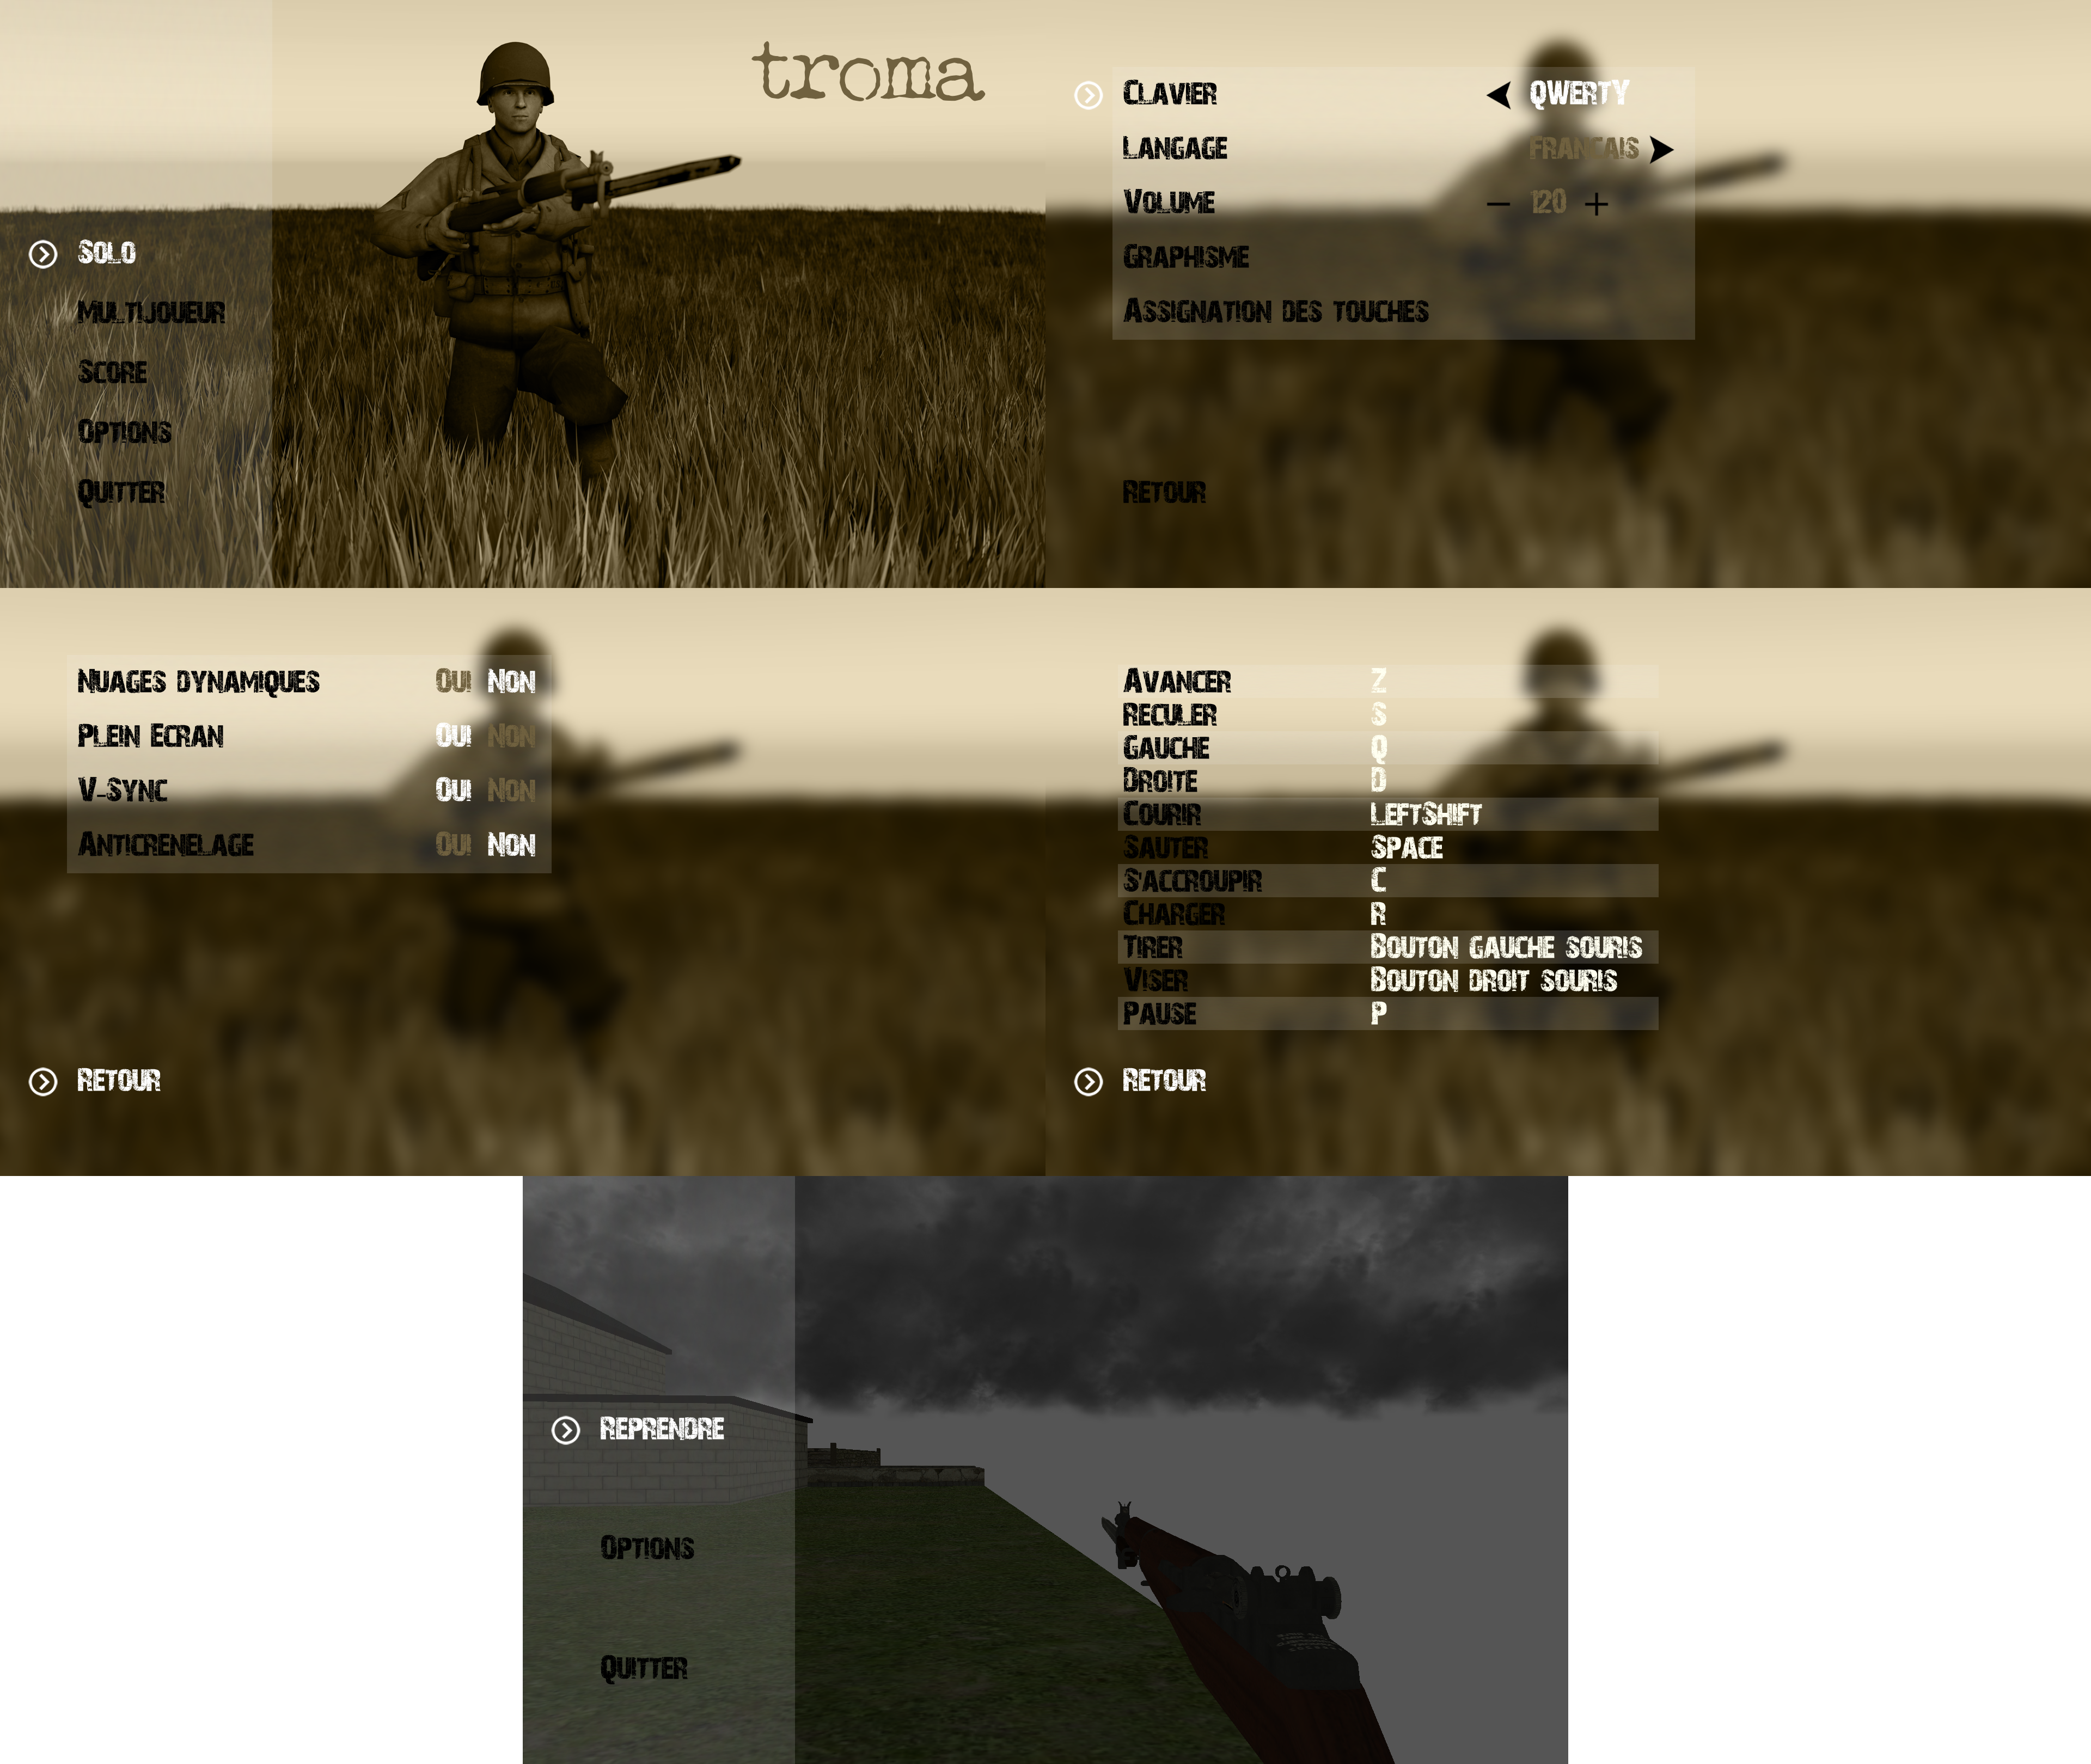
\includegraphics[width=11cm]{menu-3.png}
\caption{Captures d'écran de plusieurs menus à la fin du projet}
\end{figure}

Le design retenu suit la tendance actuelle dans le monde du jeu vidéo. C'est-à-dire un menu épuré, très sobre et s'accordant parfaitement avec notre jeu. L'idée principale repose sur un fond d'écran mettant en scène notre personnage 3D ainsi que son arme, des bandes blanches semi-transparentes ainsi que l'application de flou gaussien.

Pour compléter cette interface, nous avons rajouté un écran de chargement qui évite à l'utilisateur d'avoir des ralentissements au lancement du jeu.

\section{Vidéos d'introduction}

Notre projet étant un jeu de guerre, nous voulions pouvoir informer les utilisateurs, dès le lancement du jeu, d'un âge conseillé. Ainsi nous avons choisi d'utiliser les logo de la l'agence PEGI\footnote{Pan European Game Information} dans une très courte vidéo avertissant les joueurs au lancement du jeu.

\begin{figure}[htbp]
\centering
\includegraphics[width=8cm]{pegi18.png}
\caption{Capture d'écran du PEGI 18}
\end{figure}

Pour compléter le démarrage de notre jeu, nous avons mis à profit nos différents talents artistiques pour réaliser, avec blender, une vidéo d'introduction de notre studio. Cette vidéo devait être courte et marquer les esprits.

Le fil conducteur de cette introduction est une grenade qui explose au ralenti. La caméra change régulièrement d'angle de vue jusqu'à revenir à sa position initiale. A ce moment là, l'explosion reprend à sa vitesse normale et on voit apparaître le texte ``Emagine Studio''.

\begin{figure}[htbp]
\centering
\includegraphics[width=11cm]{anim-eie.png}
\caption{Ensemble de captures d'écran de l'animation}
\end{figure}

Grâce à ces petits ajouts au lancement du jeu, nous sommes passés d’un jeu amateur à un jeu s'approchant au maximum de ceux sur le marché.

\section{HUD}

Jusqu'à la soutenance 2, notre jeu était complètement dépourvu d'affichage tête haute\footnote{HUD : Head up display}. En effet notre vision du jeu était tournée vers le rapprochement au maximum de la réalité. Un HUD aurai donc rajouté des informations qu'un soldat pendant la seconde guerre mondiale n'aurait pas forcément eu.

Cependant, nos premiers joueurs nous ont très rapidement remonté un désaccord avec notre vision du jeu. Il nous a donc fallu nous adapter et penser à une interface simple mais comportant les informations demandées par les utilisateurs.

\begin{figure}[htbp]
\centering
\includegraphics[width=8cm]{hud.png}
\caption{Capture d'écran du HUD en mode solo}
\label{hud}
\end{figure}

Notre jeu possède deux affichages tête haute, une pour le mode solo et une pour le mode multijoueur. Ceux-ci sont presque identiques à une ou deux informations près. Comme on peut le voir sur la figure~\ref{hud}, l'interface se divise en trois parties. En haut à gauche on retrouve le temps écoulé depuis le début de la partie. En haut à droite on retrouve, ici en mode solo, le nombre de cibles restantes sur la carte. Et enfin, en bas à droite, on retrouve le nom de l'arme ainsi que le nombre de munitions et de chargeurs disponibles.

\chapter{Audio}

Dans un jeu vidéo, les effets sonores sont aussi importants que le rendu visuel. En effet pour pouvoir s'immerger dans le contexte audio, notre cerveau a besoin d'un retour auditif de ces actions.

Le travail mené sur cette partie à principalement été réalisé en deux parties : l'implémentation d'un gestionnaire des effets sonores et des musiques, et la recherche de bandes sonores appropriées. Pour cette deuxième partie, nous avons passé la plupart de notre temps à faire des recherches sur YouTube et FreeSound\footnote{\url{http://www.freesound.org/}}, un catalogue en ligne de sons libres et gratuits.

\section{La musique de fond}

La musique de fond est activé lors de la navigation dans les différents menus. Celle-ci permet de donner vie à l'interface épurée. Nous avons pris soin de choisir une musique sur le thème de la guerre pour toujours coller à l'histoire du jeu.

\section{Les effets sonores}

Plusieurs effets sonores sont disponibles dans le jeu. On en retrouve dans les menus, lors de la navigation entre les différents boutons ou encore lors de la validation d'une action. Par exemple lorsqu'on appuie sur un bouton ou que l'on change un réglage, on a un retour sonore de l'action.

On retrouve également des effets sonores dans le jeu en lui même. Tout d'abord lors des mouvements du personnage. Nous avons essayé de reproduire un son réaliste des mouvements, lorsque la personne marche ou coure. Mais également dans les actions que le joueur exécute : tirer, recharger, etc.

Ainsi le joueur devrait être toujours un peu plus immergé dans le jeu.

\chapter{Gameplay}

Le gameplay regroupe un ensemble de fonctionnalité qui forme le jeu finale, telles que les actions possibles du joueur et les modes de jeu.

\section{Les actions possibles}

Le personnage peut se déplacer à partir des touches Z, Q, D, S qui représentent respectivement avancer, gauche, droite et reculer (sur un clavier AZERTY). Les touches marchent par paire : Z et S, Q et D. C'est-à-dire que si vous appuyez sur les deux touches d'une paire en même temps le mouvement s'annule. En effet il est difficile d'aller à droite tout en allant à gauche. Il est également intéressant de noter que nous gérons les mouvements en diagonales. De plus lors d'un mouvement, le maintien de la touche Z (avancer) et de la touche SHIFT gauche permet de courir.

\begin{figure}[htbp]
\centering
\includegraphics[width=8cm]{viser.png}
\caption{Capture d'écran du mode visé}
\end{figure}

Le joueur peut également déplacer la souris afin de changer l'angle de la caméra. Pour se faire, nous calculons à chaque fois la différence entre la position d'origine et la nouvelle position du curseur de la souris sur l'écran. Nous appliquons alors un coefficient à cette différence afin d'amplifier le mouvement.

Deux autres mouvements sont possibles : s'accroupir et sauter. Ils sont respectivement représentés sur le clavier par les touches C et ESPACE.

A ces mouvements s'ajoutent des actions indispensables dans un FPS : tirer, viser et recharger. Elles sont respectivement déclenchées par un clique gauche, un clique droit et l'appuie de la touche R.

Nous avons fait le choix de rendre le jeu jouable à la manette. L'ensemble de ces actions sont donc accessible par des touches de la manette d'Xbox 360.

\section{Modes de jeu}

Notre jeu se compose de deux modes de jeu : le mode solo et le mode multijoueur. Le mode solo est un mode d'entrainement afin d'améliorer les réflexes du joueur pour ses futurs parties multijoueurs. Il consiste à détruire l'ensemble des cibles sur le terrain le plus rapidement possible. Une fois que toutes les cibles sont détruites, la partie s'arrête et affiche le temps mis par le joueur.

\begin{figure}[htbp]
\centering
\includegraphics[width=8cm]{score.png}
\caption{Capture d'écran d'une fin de partie en mode solo}
\end{figure}

Le mode multijoueur est un chacun pour soi. Les parties durent dix minutes. Pendant ce laps de temps, chaque joueur s'affronte afin d'arriver premier dans le classement. Pour ce mode, nous avons tenté de concevoir un terrain qui favorise les affrontements au maximum.


\chapter{Réseau}

L'implémentation du réseau dans notre jeu à commencé après la soutenance 1. Le réseau est à l'origine de nombreuses modifications du fonctionnement de notre moteur de jeu. Mais avant de pouvoir commencer l'implémentation, il nous a fallu concevoir une architecture réseau et définir les différentes communications qui seront nécessaires.

\section{La structure}

\subsection{La connexion}

Ce que nous appelons ici connexion, c'est lorsque le joueur lance le mode multijoueur dans le jeu. Le jeu cherche alors à établir une connexion entre le client et un serveur principal que nous hébergeons chez OVH\footnote{OVH est un hébergeur français, \url{http://www.ovh.com/fr/index.xml}}. Ce serveur principal maintient une liste des joueurs connectés et leur attribut un ID unique. De plus, celui-ci fait la même chose avec les parties lancées.

Une fois que la connexion est établie et que le joueur possède un identifiant, le serveur lui envoie la liste des parties disponibles. Le joueur peut alors rejoindre une partie ou en créer une nouvelle.

Si le client décide de rejoindre une partie, il va tenter d'établir une connexion avec le serveur qui l'héberge. On appelle ce dernier hôte. En effet il s'agit d'un ordinateur sur lequel tourne la partie client et serveur du jeu. Cette technique nous permet d'éviter la surcharge de notre serveur central.

Si le client décide de créer une nouvelle partie, il devient automatiquement hôte. C'est-à-dire que la partie serveur du jeu démarrera sur son ordinateur. L'hôte est le seul ordinateur en partie qui maintient une connexion avec le serveur central afin de faire remonter régulièrement des informations sur la partie en cours, telle que le nombre de joueur dans la partie. La communication entre les clients et l'hôte est expliquée dans le paragraphe suivant.

Cette connexion entre le serveur central et les clients/hôtes est réalisée à partir du protocole TCP\footnote{Transmission Control Protocol}. En effet, nous avons besoin ici d'une confirmation que l'ensemble des informations soient correctement transmisses.

\subsection{Les communications durant une partie}

Nous avons choisi d'implémenter une architecture client-serveur. Le serveur, qui est donc ici l'hôte et non pas le serveur central, est chargé de recevoir l'ensemble des entrées de tous les joueurs et faire le calcul de la physique ainsi que de la logique du jeu. Une fois les calculs effectués, le serveur renvoie l'ensemble des résultats à l'ensemble des joueurs.

De leur côté, les clients s'occupent d'envoyer l'ensemble des entrées au serveur ainsi que de faire des calculs de physique approximative. Ainsi le joueur ne devrait pas être gêné par le temps de latence entre lui et le serveur. Les résultats des calculs effectués par le serveur permettent aux clients de corriger les approximations afin de rester un maximum synchronisé avec le serveur. C'est ce qu'on appelle la technique du ``client side prediction''. Si le client se retrouve totalement désynchronisé par rapport au serveur, par exemple après une perte de paquets trop importante, le serveur utilise sa temporisation des calculs pour envoyer une commande au joueur avec la position à laquelle il doit se repositionner pour être synchronisé.

Pour mieux comprendre le fonctionnement, vous pouvez vous référer à la figure~\ref{reseau}. Au centre de celle-ci repose sur un socle bleu l'hôte de la partie. Les autres ordinateurs portables représentent les différents clients. En haut à droite, on y trouve un regroupement de serveurs (en couleur gris). Celui-ci représente notre serveur central. Les différentes connexions et communications sont matérialisées par un trait bleu.

\begin{figure}[htbp]
\centering
\includegraphics[width=8cm]{reseau.jpg}
\caption{Schéma illustrant les communications durant une partie}
\label{reseau}
\end{figure}

Bien entendu pour réaliser l'ensemble de ces concepts, nous nous sommes basés sur le protocole UDP\footnote{User Datagram Protocol}. Il s'agit d'un protocole de transport de la pile de protocole TCP/IP qui fonctionne sans connexion préalable, par rapport au TCP. Ainsi le protocole UDP ne garantit pas la bonne transmission des données, ni l'ordre d'arrivée. Cependant ce protocole à l'avantage d'être le plus rapide. En effet si un paquet est perdu, le client n'est pas obligé d'attendre que le serveur le renvoi, il recevra directement les paquets suivants. Ainsi il n'y pas de blocage du flux de données par rapport au TCP qui maintient un flux de données ordonnées dans l'ordre de transmission.

\section{Implémentation et problème}

Au niveau de l'implémentation, nous avons choisi d'utiliser la bibliothèque Lidgren\footnote{\url{https://code.google.com/p/lidgren-network-gen3/}}. Il s'agit d'une bibliothèque réseau réputée et conçu en C\#.

Bien que cette bibliothèque soit robuste et possède des outils de debogage, le développement du mode multijoueur a été plus difficile que ce à quoi nous nous attendions. Nombreux sont les problèmes que nous avons rencontrés et que nous avions du mal à identifier. En effet il est très difficile de comprendre l'origine des différents bugs. Pour cela, nous avons dû développer des outils pour garder une trace compréhensible des connexions établies et des différentes communications.

Malgré ces outils, le fonctionnement de notre mode multijoueur est encore assez aléatoire. Il peut fonctionner correctement ou cesser de fonctionner en plein milieu d'une partie. Nous nous efforçons encore aujourd'hui de le rendre le plus stable possible pour notre soutenance finale.

\chapter{Site web}

\section{La conception du design}

Pour la conception du site web, un petit challenge entre Thibault et Rémy a été organisé. Ils devaient concevoir de leur côté un design complet du site. Le gagnant sera alors celui dont le design plaira le plus au reste de l'équipe et à un petit groupe d'amis.

Ils ont alors chacun conçu des designs sur papier puis réalisé une première ébauche du site. Une seule limitation leur était imposée : le site devait être ``responsive desgin''. C'est à dire qu'il doit s'adapter à toutes les tailles d'écrans : ordinateur de bureau, ordinateur portable, tablette et smartphone.

Il n'y a eu finalement aucun gagnant. Thibault et Rémy ont préféré fusionner leur deux visions différentes pour créer le design actuel de notre site web. Ceci est encore une démonstration de notre capacité à fonctionner en équipe.

Le site a été conçu avec Foundation, un framework HTML/CSS/Javascript qui permet de concevoir très rapidement des sites internet avec de nombreuses fonctionnalités. Mais le grand intérêt de ce type de framework c'est qu'ils sont pensés pour être ``responsive design'' et qu'ils s'affichent à l'identique sur l'ensemble des navigateurs internet. Un avantage de Foundation par rapport à ces concurrents est une plus grande facilité de personnalisation du design de base. Tout est pensé pour obliger le développeur à y intégrer sa propre vision.

\section{Contenu et accès au site internet}

Le site web comporte différentes parties, dont :

\begin{itemize}
  \item l’histoire du personnage principal dans le jeu, afin de donner envie au visiteur de télécharger et de jouer à notre jeu.
  \item une rubrique actualité pour pouvoir être informé des différentes évolutions du projet
  \item un ensemble de captures d'écran régulièrement actualisées
  \item la présentation de notre équipe, avec des photos et de petites descriptions.
  \item la progression actuelle de la conception de notre jeu
  \item une partie téléchargement permettant d'obtenir les rapports des soutenances, le jeu et des fonds d'écran
  \item un ensemble d'information pour nous contacter par mail ou sur les réseaux sociaux.
\end{itemize}

Notre site internet est accessible à l'adresse \url{http://www.troma.eu/}. A partir de celui-ci vous pouvez avoir accès aux réseaux sociaux sur lesquels nous essayons d'être régulièrement actif !

\section{Bref résumé des actualisations}

Le site a été actualisé à de nombreuses reprises, mais certaines actualisations sont plus importantes que d'autres. Par exemple, après la soutenance 1, nous avons introduit une nouvelle rubrique actualité permettant aux visiteurs d'être informées de l'évolution du projet.

Après la soutenance 2, l'équipe a réactualisé l'ensemble du contenu du site (captures d'écran, textes, etc) et mis en ligne la nouvelle version du jeu. Peu de temps après, nous avons réalisé des fonds d'écran mettant en scène le personnage de notre jeu. Ceux-ci sont disponibles dans la partie téléchargement et ont une résolution maximale de 8K ! Pour la petite anecdote, ce rendu 3D a été réalisé sur une ferme de serveur, spécialisée dans le calcul numérique, en 4h. Sur l'ordinateur d'un particulier, celui-ci aurai mis entre 24 à 48h.

Après la soutenance finale, nous actualiserons notre site internet afin de mettre en ligne la version finale du jeu.

\begin{figure}[htbp]
\centering
\includegraphics[width=13cm]{site_web.png}
\caption{Notre site web, le 29/05/14}
\end{figure}

\chapter{Synthèses personnelles}

\section{Thibault}

Je suis passionné d’informatique depuis la cinquième. Cette passion m’a permis de développer très rapidement de nombreuses connaissances, notamment en m’impliquant dans des projets libres mais également par le biais de ma première et terminal S SI où j’ai été amené à diriger deux projets conséquents. De mes expériences antérieures, j’ai appris que chaque projet était un apport de connaissance très important, mais aussi qu’il doit être dirigé pour ne pas divaguer. C’est pourquoi je me suis rapidement proposé comme chef de projet. Je pensais avoir la capacité et l’expérience nécessaire pour mener à bien le groupe.

Le développement 3D est un sujet complexe et très vaste. Il est impossible de le parcourir dans son intégralité en seulement six mois. Il fallait donc posé dès le départ des limites, afin de ne pas perdre de temps à faire des recherches qui n’aboutiraient à rien. Notre première organisation a donc été de fixer les lignes de notre projet, mais également les différents bonus possibles. Ensuite nous avons pris soin de partager les tâches entre chacun des membres. J’ai fait en sorte de respecter les préférences de chacun mais également d’attribuer à chaque fois deux personnes sur chaque tâches. Ainsi, si quelqu’un a un problème ou perds en motivation, son binôme peut prendre le relais, l’aider et le remotiver.

La motivation est un facteur clé dans un projet de cette durée. En effet, sans motivation un groupe n’avance pas et se retrouve rapidement en retard sur son planning. Or notre but était de ne surtout pas devoir travailler d’arrache-pied la veille d’une soutenance. Nous avons donc essayé de rester motiver au maximum. Pour ceci j’ai utilisé une petite astuce tirée de la méthode de développement agile SCRUM. Celle-ci consiste à alterner le type de tâches réalisées. Il y en a principalement deux : celles dites d’arrière-plans, c’est-à-dire nécessaires mais qui n’apportent aucun résultat visible pour l’utilisateur, et celles dites de premier-plans qui apportent un résultat concret à l’utilisateur. Or durant le développement d’un projet, le développeur est l’utilisateur numéro un du celui-ci. Ainsi dans notre planning, j’ai en permanence alterné ces deux types de tâches pour motiver au maximum l’équipe. Et si le projet n’avançait pas, je réalisais l’une des tâches de premier-plan afin de redonner envie au membre de mon équipe de travailler sur le projet.

Le planning, la répartition des tâches et la motivation nous ont permis d’avancer rapidement et de prendre de l’avance pour résoudre nos problèmes. Notre fonctionnement peut s’apparenter un peu à celui d’une jeune start-up. Nous expérimentons, nous nous améliorons et nous tentons d’être le plus productif et le plus professionnel possible. Et je pense que nous avons plutôt bien réussi à mener notre projet à terme.

De manière plus personnelle, je suis d’abord très fier en tant que chef de projet du résultat obtenu et de l’équipe que j’ai eu à mener. Bien que ce poste m’ait apporté une charge de travail supplémentaire, j’ai apprécié les responsabilités qui m’ont été confié, telles que la gestion du planning, la résolution des conflits, l’aide de l’ensemble des membres du groupe, etc. Je pense que cette expérience me sera très utile dans ma futur vie professionnelle où je serai probablement amené à diriger une équipe ou/et un projet.

Je suis également satisfait des nombreuses connaissances que j’ai pu apprendre, notamment dans le domaine du réseau et de la 3D. Et même si celles-ci ne me seront pas forcément utiles dans ma carrière, je suis persuadé qu’elles me permettront de m’adapter plus facilement.

Pour conclure, je dirai que ce projet de six mois aura été éprouvant par le rythme qu’il impose, mais qu’en contrepartie il constitue une expérience très riche qui me servira tout au long de mes études et de ma carrière professionnelle.

\section{Rémy}

Novice dans le domaine de l'informatique, je pense que le projet est un bon moyen de s'améliorer en programmation. Durant ce projet, j'ai été en charge du son, du menu, du gameplay ainsi que du site web. Je ne suis pas le programmeur fou mais je me débrouille à ma manière pour réussir à faire avancer le projet.

C’est un groupe très dynamique où chaque personne du groupe s’entend avec les autres, j’ai bien aimé cet aspect la car on peut observer que dans certains autres groupes, l’égo de chacun prend le dessus et cela peut vite devenir l’anarchie.

Nous nous sommes très bien répartis les tâches. Les personnes qui savent le mieux codé font de la programmation un peu plus poussé, complexe (surtout Thibault Deutsch qui a un très bon niveau en programmation) pour permettre d’avoir un meilleur rendu visuel (tel que les particules pour les nuages où nous sommes tous restés bouche bée devant ce qu’il a fait). Ce qui nous permet aussi d’apprendre en regardant ce qu’il fait.

Chaque personne à son mot à dire et nous demandons l’avis du groupe pour soit supprimer ou garder quelque chose dans le projet. Si il y a toujours conflit, nous nous sommes mis d’accord au début d’année que ce soit le chef de projet qui tranche sur le sujet. Ce qui rend un peu plus notre projet comme une start up avec toutes les personnes du projet qui travail mais une personne qui a une part de responsabilité en plus.
Nous avons eu des problèmes tout au long du projet avec des parties qui ne s’implémentaient pas et qu’on devait absolument résoudre avant les soutenances. Des moments de stress plus intense que d’habitude qui ne nous aide pas beaucoup à l’avance du projet.

J’ai rencontré des difficultés sur certaine de mes parties, non pas parce que je ne savais pas comment faire, parce que je ne connaissais pas le langage approprié car je ne l’avais pas appris. Il a donc fallu aller se documenter sur internet et faire quelques exercices pratiques pour essayer de comprendre et de voir comment cela fonctionne.

J’ai beaucoup appris grâce à ce projet, que ce soit le travail en groupe, la répartition des tâches ou même d’avoir un projet à rendre comme en entreprises. Par rapport au travail en groupe je dois dire que c’est une très bonne chose de l’avoir expérimenté car dans beaucoup d‘entreprise, plusieurs personnes sont réunis sur un même projet. Ce qui signifie qu’une personne ne fait pas le projet seul, ils doivent se répartir les rôles, les tâches, qui fait quoi, et cela est très enrichissant car ce n’est pas si simple que cela quand tout est mal organisé dès le début. On doit surtout se comprendre entre nous, car l’incompréhension amène souvent les personnes à faire quelque chose qui n’était pas prévu par le groupe ou qui était déjà fait par quelqu’un d’autre et cela joue beaucoup sur le planning. On ne travaille pas tous en même temps donc il faut souvent faire des réunions ou se briefer pour voir qui est dans les temps sur ses parties ou non. J’ai bien aimé le fait qu’on puisse s’entraider mutuellement, si j’ai un problème sur une partie je peux demander à quelqu’un du groupe comment il aurait fait pour résoudre ce problème car on n’a pas tous la même vision des choses, et la plupart du temps cela fonctionne car la personne a pris le problème sous un autre angle.

Le projet m’a vraiment appris beaucoup que ce soit en termes de travail en groupe, ou en apprentissage personnel en programmation. Il m’a permis de respecter un planning et de ne pas reporter ce que j’avais à faire au lendemain pour ne pas retarder le groupe, car les parties sont liées entre-elles et cela entrainerait un retard pour le tout le groupe. 


\section{Marc}

Passionné d’informatique depuis mon enfance, j’ai toujours souhaité comprendre le fonctionnement d’un ordinateur ; aussi bien du côté matériel que logiciel. Le projet à réaliser en première année à l’EPITA m’a permis de répondre à ce besoin.

La conception d’un logiciel, en l’occurrence d’un jeu est une façon très stimulante pour apprendre et comprendre la programmation. La motivation pour mener à bien ce projet m’a permis d’acquérir une aisance vis-à-vis de la programmation orientée objet, mais aussi une nouvelle expérience de travail en groupe.

L’organisation que nous avons choisie fut de répartir différentes parties à un ou plusieurs membres afin de permettre une avancé rapide. Cependant nous avons eu l’occasion d’apporter aide, avis ou conseil aux autres membres.  Je me suis principalement occupé de la partie graphique et du réseau. En dehors de la programmation en elle-même, j’ai beaucoup appris sur la conception et le rendu d’objet en 3 dimensions en informatique, mais aussi sur la structure des réseaux et leur fonctionnement. Les difficultés majeures que j’ai rencontrées concernaient l’export des modèles et leur utilisation dans XNA. Heureusement j’ai pu trouver de l’aide soit sur des forums ou dans la documentation officielle soit auprès d’autres étudiants au sein du groupe ou de l’école. Les nombreux problèmes que nous avons pu rencontrer nous ont parfois démoralisé mais jamais découragé et nous avons toujours réussi à trouver des solutions. C’est ce que je retiens de cette expérience : ``Un problème sans solution est un problème mal posé'', Albert Einstein.

Concernant le groupe, nous avons su travailler en équipe et nous entraider. Je garde un bon souvenir de cette expérience qui m’a beaucoup apportée. Elle est indispensable pour une future insertion dans le milieu professionnel où savoir travailler en groupe est primordial.

Ce projet est le plus long et le plus élaboré que j’ai à mon actif mais c’est surtout le premier que j’ai réalisé en groupe. Il est le premier d’une longue série et m’a convaincu que j’avais fait le bon choix en venant à l’EPITA. En association des cours plus théoriques, les TP et les projets que nous avons à réaliser nous offrent une véritable expérience informatique. Bien que je n’ai pas vocation à travailler dans le domaine vidéo-ludique, j’ai beaucoup apprécié ces 6 mois de développement.

\section{Anthony}

L'idée de partir de zéro et de tout construire soit même m'a toujours beaucoup plu ainsi depuis le début je suis très motivé par ce projet non seulement car il s'agit de créer mon premier jeu mais également car je pense que nous pouvons aboutir à quelque chose de très convaincant.

Dans un premier temps j'ai vu ce projet comme un moyen d'apprendre à mener à bien une idée, de créer un produit. Cependant au fil du temps je me suis aperçu qu'il s'agissait de beaucoup plus que ça. La première chose qu'il faut savoir gérer, et à laquelle je n'avais pas forcement pensé au début est le travail en groupe, non seulement pour le chef de projet mais également pour le reste de l'équipe. Et cela nous amène directement au second point: la gestion du temps.

Je me suis rendu compte que ces deux points étaient reliés lorsqu'il a fallu avancer rapidement et en peu de temps sur notre travail! Il est apparu clair que nous devions optimiser notre temps et chacun s'est mis à travailler conjointement sur une partie du jeu.

Ainsi la répartition des taches et le travail régulier sont devenu les deux clés pour mener à bien notre projet.

Enfin, plus personnellement ce projet m'a apporté des nombreuses connaissances en C\# et plus globalement en programmation. J'ai appris différentes ``techniques''  sur la mise en place d'un projet, de 3D, d'interface... ceci étant applicables à n'importe quel langage! Et je pense que c'est ça le plus important, il faut apprendre des choses qui nous servirons pour le futur car la forme a, certes, de l'importance mais le fond en a doublement!

\chapter*{Conclusion}

Le projet Troma a débuté en janvier 2014, nous avions l'objectif de réaliser un jeu de guerre sous le thème de la Seconde Guerre Mondiale. Le groupe est formé de quatre étudiants en première année sans connaissance préalable particulière en langage C\#. Cependant nous avons décidé dès le début de donner notre maximum en choisissant un jeu en 3D muni d'un mode de jeu en ligne ! 

Durant toute la phase de développement nous avons essayé de garder cet état d'esprit qui est de toujours donner le maximum. Les notes que nous avons obtenues aux deux premières soutenances nous ont encourager à continuer dans cette voie. Nous avons donc implémenter toutes les fonctionnalités du jeu une par une avec plus ou moins de difficulté mais sans jamais abandonner même quand cela s'avérait beaucoup plus difficile que prévu. L'aspect technique n'a pas été la seule difficulté, le côté organisationnel des soutenances et du planning à respecter pour l'équipe en a aussi été une! Notre point fort a été de ne jamais attendre le dernier moment et d'essayer de prendre le maximum d'avance possible sur notre planning prévisionnel lorsque cela était possible.

Aujourd'hui nous sommes fiers d'avoir réussi à mener à bien notre projet de bout en bout. Cette expérience a été très enrichissante pour chacun d'entre nous. Nous pensons que ce travail de groupe nous permettra d'aborder avec plus de facilité nos futurs projets à l'EPITA et/ou en entreprise.

\newpage
\pagenumbering{Roman}
\part*{Annexes}

\bibliographystyle{plain}
\nocite{*}
\bibliography{bibliographie}

\newpage
\listoffigures

\newpage
\tableofcontents
 
\end{document}